\documentclass[12pt,a4paper]{article}

% ─── Page Layout ───────────────────────────────────────────────────────────────
\usepackage[a4paper, margin=0.8in, headheight=14pt]{geometry}

% ─── Fonts (XeLaTeX) ───────────────────────────────────────────────────────────
\usepackage{fontspec}
\usepackage{unicode-math}
\setmainfont{TeX Gyre Pagella}
\setmonofont[Scale=0.88]{TeX Gyre Cursor}
\setmathfont{Latin Modern Math}

% ─── Packages ──────────────────────────────────────────────────────────────────
\usepackage{xcolor}
\usepackage{colortbl}
\usepackage{titlesec}
\usepackage{enumitem}
\usepackage{tabularx}
\usepackage{booktabs}
\usepackage{array}
\usepackage{amsmath}
\usepackage{tikz}
\usetikzlibrary{shapes.geometric, arrows.meta, positioning, calc, fit, decorations.pathreplacing, decorations.pathmorphing}
\usepackage{tcolorbox}
\tcbuselibrary{skins, breakable}
\usepackage{hyperref}
\usepackage{fancyhdr}
\usepackage{graphicx}
\usepackage{microtype}
\hyphenpenalty=10000
\exhyphenpenalty=10000
\sloppy
\usepackage{caption}
\usepackage{setspace}
\usepackage{multirow}
\usepackage{tocloft}

% ─── Q&A helper ────────────────────────────────────────────────────────────────
\newcommand{\Q}[1]{\textbf{#1}\par\noindent\ignorespaces}

% ─── Colour Palette ────────────────────────────────────────────────────────────
\definecolor{myred}{RGB}{196,30,58}
\definecolor{mydark}{RGB}{30,30,50}
\definecolor{mygreen}{RGB}{14,120,80}
\definecolor{myteal}{RGB}{0,130,140}
\definecolor{myamber}{RGB}{180,100,0}
\definecolor{mypurple}{RGB}{100,30,160}
\definecolor{mygray}{RGB}{246,247,249}
\definecolor{mgframe}{RGB}{180,185,200}
\definecolor{watermark}{RGB}{145,150,170}
\definecolor{hdrred}{RGB}{250,232,235}
\definecolor{hdrgreen}{RGB}{220,244,233}
\definecolor{hdrteal}{RGB}{220,242,244}
\definecolor{hdramber}{RGB}{253,242,215}
\definecolor{hdrpurple}{RGB}{238,228,255}
\definecolor{hdrgray}{RGB}{238,240,245}
\definecolor{rowalt}{RGB}{250,251,253}

% ─── Section Formatting ────────────────────────────────────────────────────────
\titleformat{\section}
  {\large\bfseries\color{myred}}{\thesection.}{0.5em}{}
  [\vspace{1pt}{\color{myred}\rule{\linewidth}{0.8pt}}]
\titleformat{\subsection}
  {\normalsize\bfseries\color{myteal}}{\thesubsection}{0.5em}{}
\titlespacing*{\section}{0pt}{18pt}{7pt}
\titlespacing*{\subsection}{0pt}{11pt}{4pt}

% ─── Paragraph ─────────────────────────────────────────────────────────────────
\setlength{\parindent}{0pt}
\setlength{\parskip}{4pt}

% ─── TOC Styling ───────────────────────────────────────────────────────────────
\renewcommand{\cfttoctitlefont}{\large\bfseries\color{myred}}
\renewcommand{\cftaftertoctitle}{\par\noindent{\color{myred}\rule{\linewidth}{0.8pt}}}
\setlength{\cftbeforetoctitleskip}{0pt}
\setlength{\cftaftertoctitleskip}{6pt}
\renewcommand{\cftsecfont}{\normalsize\bfseries\color{mydark}}
\renewcommand{\cftsecpagefont}{\normalsize\bfseries\color{mydark}}
\renewcommand{\cftsecleader}{\cftdotfill{\cftdotsep}}
\setlength{\cftbeforesecskip}{7pt}
\renewcommand{\cftsubsecfont}{\small\color{mydark}}
\renewcommand{\cftsubsecpagefont}{\small\color{mydark}}
\setlength{\cftbeforesubsecskip}{3pt}
\setlength{\cftsubsecindent}{1.4em}

% ─── Table helpers ─────────────────────────────────────────────────────────────
\renewcommand{\arraystretch}{1.45}
\setlength{\tabcolsep}{6pt}
\arrayrulecolor{mydark}
\newcolumntype{B}[1]{>{\small\bfseries\raggedright\arraybackslash}m{#1}}
\newcolumntype{C}[1]{>{\centering\arraybackslash}m{#1}}
\newcolumntype{Y}{>{\small\raggedright\arraybackslash}X}
\renewcommand{\tabularxcolumn}[1]{m{#1}}

% ─── Header / Footer ───────────────────────────────────────────────────────────
\pagestyle{fancy}
\fancyhf{}
\fancyhead[L]{\small\color{myred}\textbf{OE-EC704A}\;\color{mydark}--- Web Technology}
\fancyhead[R]{\small\color{myteal}\textbf{Module 2 Notes}}
\fancyfoot[C]{\small\color{mydark}\thepage}
\fancyfoot[R]{\small\color{watermark}\textit{\copyright\ Biraj}}
\renewcommand{\headrulewidth}{0.5pt}
\renewcommand{\footrulewidth}{0.3pt}

% ─── Hyperref ──────────────────────────────────────────────────────────────────
\hypersetup{
  colorlinks=true, linkcolor=myteal, urlcolor=myteal,
  pdfauthor={Biraj Sarkar},
  pdftitle={OE-EC704A --- Module 2 Notes}
}

% ─── tcolorbox styles ──────────────────────────────────────────────────────────
\tcbset{
  tikzbox/.style={
    colback=mygray, colframe=mgframe, boxrule=0.6pt, arc=4pt,
    left=8pt, right=8pt, top=6pt, bottom=6pt,
    colbacktitle=mgframe, coltitle=mydark,
    fonttitle=\small\bfseries
  },
  defbox/.style={
    colback=hdrgreen, colframe=mygreen, boxrule=0.8pt, arc=4pt,
    left=9pt, right=9pt, top=6pt, bottom=6pt,
    colbacktitle=mygreen, coltitle=white,
    fonttitle=\small\bfseries
  },
  formulabox/.style={
    colback=hdrteal, colframe=myteal, boxrule=0.8pt, arc=4pt,
    left=9pt, right=9pt, top=7pt, bottom=7pt,
    colbacktitle=myteal, coltitle=white,
    fonttitle=\small\bfseries
  },
  examplebox/.style={
    colback=hdramber, colframe=myamber, boxrule=0.8pt, arc=4pt,
    left=9pt, right=9pt, top=6pt, bottom=6pt,
    colbacktitle=myamber, coltitle=white,
    fonttitle=\small\bfseries
  },
  masonbox/.style={
    colback=hdrpurple, colframe=mypurple, boxrule=0.8pt, arc=4pt,
    left=9pt, right=9pt, top=6pt, bottom=6pt,
    colbacktitle=mypurple, coltitle=white,
    fonttitle=\small\bfseries
  },
  exambox/.style={
    colback=hdrpurple, colframe=mypurple, boxrule=1pt, arc=5pt,
    left=10pt, right=10pt, top=8pt, bottom=8pt,
    colbacktitle=mypurple, coltitle=white,
    fonttitle=\bfseries,
    breakable, title after break={\textbf{Frequently Asked / Viva Questions (contd.)}}}
}
\tcbset{breakable}

% ─── TikZ styles ───────────────────────────────────────────────────────────────
\tikzset{
  block/.style={rectangle, draw=myteal, fill=hdrteal,
    text width=2.5cm, align=center, minimum height=1.0cm,
    font=\small, rounded corners=3pt, line width=0.7pt},
  redblock/.style={rectangle, draw=myred, fill=hdrred,
    text width=2.5cm, align=center, minimum height=1.0cm,
    font=\small, rounded corners=3pt, line width=0.7pt},
  netnode/.style={rectangle, draw=myteal, fill=hdrteal,
    text width=1.8cm, align=center, minimum height=0.8cm,
    font=\small, rounded corners=3pt, line width=0.7pt},
  sumjunc/.style={circle, draw=myamber, fill=hdramber,
    minimum size=0.6cm, font=\small, line width=0.8pt},
  snode/.style={circle, draw=mypurple, fill=hdrpurple,
    minimum size=0.55cm, font=\footnotesize, line width=0.7pt},
  arrow/.style={-Stealth, thick, color=mydark},
  redarrow/.style={-Stealth, thick, color=myred},
  line/.style={thick, color=mydark}
}

% ═══════════════════════════════════════════════════════════════════════════════
\begin{document}
% ═══════════════════════════════════════════════════════════════════════════════

\begin{center}
  {\LARGE\bfseries\color{myred} OE-EC704A --- Web Technology}\\[5pt]
  {\normalsize\color{mydark} Semester VII \quad$\bullet$\quad 3L:0T:0P \quad$\bullet$\quad 3 Credits}\\[3pt]
  {\normalsize\color{myteal}\textbf{Module 2 Exam Notes: Introduction to Java Programming \& OOP}}\\[3pt]
  {\small\color{mydark} CGEC \;$|$\; B.Tech ECE (2023--27) \;$|$\; \textit{Biraj Sarkar}}
\end{center}
\vspace{2pt}
\noindent{\color{myred}\rule{\linewidth}{1.5pt}}
\vspace{2pt}

\hypersetup{linkcolor=mydark}
\tableofcontents
\hypersetup{linkcolor=myteal}
\newpage

% ===============================================================================
\section{Java Execution Environment}
% ===============================================================================

Java uses a hybrid execution model combining compilation and interpretation. This ensures its core principle: \textbf{Write Once, Run Anywhere (WORA)}.

\begin{tcolorbox}[defbox, title={\textbf{Bytecode and Platform Independence}}]
\begin{itemize}[leftmargin=*, itemsep=3pt]
  \item \textbf{Bytecode:} A highly optimized set of machine instructions designed for execution by the JVM. It is stored in a \texttt{.class} file after compilation.
  \item \textbf{Platform Independence:} Java source code compiles into platform-independent bytecode. However, the \textbf{JVM itself is platform-dependent} because it must translate bytecode into the host system's native machine instructions.
\end{itemize}
\end{tcolorbox}

\begin{tcolorbox}[tikzbox, title={Java Compile-and-Run Execution Flow}]
\centering
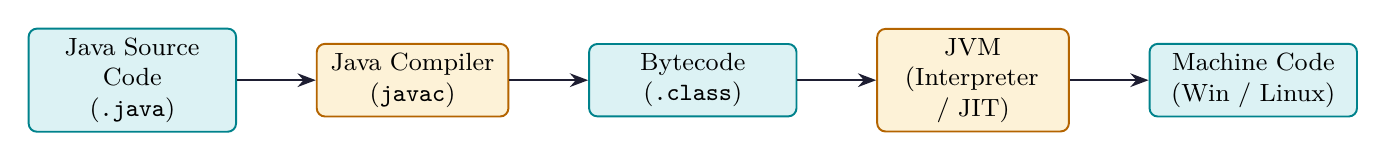
\begin{tikzpicture}[node distance=1.0cm and 1.8cm,
  node/.style={rectangle, draw=myteal, fill=hdrteal, text width=2.4cm,
    align=center, minimum height=0.9cm, font=\small, rounded corners=3pt, line width=0.7pt},
  act/.style={rectangle, draw=myamber, fill=hdramber, text width=2.2cm,
    align=center, minimum height=0.9cm, font=\small, rounded corners=3pt, line width=0.7pt}]

  % Nodes
  \node[node] (src) {Java Source Code\\(\texttt{.java})};
  \node[act, right=1.0cm of src] (compiler) {Java Compiler\\(\texttt{javac})};
  \node[node, right=1.0cm of compiler] (byte) {Bytecode\\(\texttt{.class})};
  \node[act, right=1.0cm of byte] (jvm) {JVM\\(Interpreter / JIT)};
  \node[node, right=1.0cm of jvm] (mach) {Machine Code\\(Win / Linux)};

  % Arrows
  \draw[arrow] (src) -- (compiler);
  \draw[arrow] (compiler) -- (byte);
  \draw[arrow] (byte) -- (jvm);
  \draw[arrow] (jvm) -- (mach);
\end{tikzpicture}
\end{tcolorbox}

\subsection{JDK vs. JRE vs. JVM}
Understanding the boundary between JVM, JRE, and JDK is crucial:

\begin{tcolorbox}[tikzbox, title={JDK, JRE, and JVM Containment Relationship}]
\centering
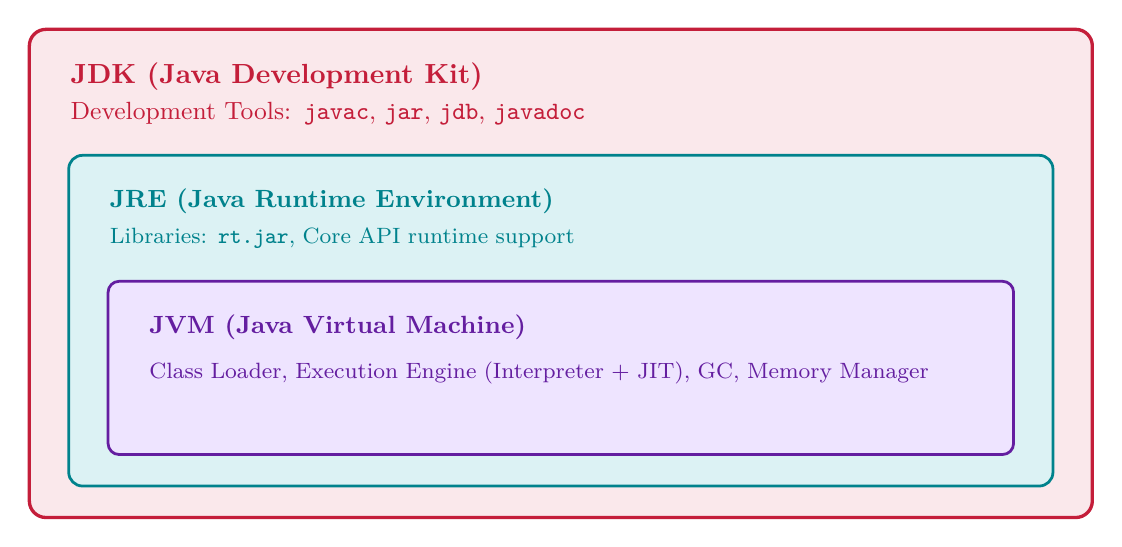
\begin{tikzpicture}
  % JDK Boundary
  \draw[draw=myred, fill=hdrred, line width=1.2pt, rounded corners=6pt] (0,0) rectangle (13.5,6.2);
  \node[anchor=north west, color=myred, font=\normalsize\bfseries] at (0.4, 5.9) {JDK (Java Development Kit)};
  \node[anchor=north west, color=myred, font=\small, align=left, text width=12.5cm] at (0.4, 5.4) {Development Tools: \texttt{javac}, \texttt{jar}, \texttt{jdb}, \texttt{javadoc}};

  % JRE Boundary
  \draw[draw=myteal, fill=hdrteal, line width=1.0pt, rounded corners=5pt] (0.5,0.4) rectangle (13.0,4.6);
  \node[anchor=north west, color=myteal, font=\small\bfseries] at (0.9, 4.3) {JRE (Java Runtime Environment)};
  \node[anchor=north west, color=myteal, font=\footnotesize, align=left, text width=11.5cm] at (0.9, 3.8) {Libraries: \texttt{rt.jar}, Core API runtime support};

  % JVM Boundary
  \draw[draw=mypurple, fill=hdrpurple, line width=1.0pt, rounded corners=4pt] (1.0,0.8) rectangle (12.5,3.0);
  \node[anchor=north west, color=mypurple, font=\small\bfseries] at (1.4, 2.7) {JVM (Java Virtual Machine)};
  \node[anchor=north west, color=mypurple, font=\footnotesize, align=left, text width=10.5cm] at (1.4, 2.1) {Class Loader, Execution Engine (Interpreter + JIT), GC, Memory Manager};
\end{tikzpicture}
\end{tcolorbox}

\par\noindent
{\renewcommand{\arraystretch}{1.5}%
\begin{tabularx}{\linewidth}{|B{3.2cm}|Y|Y|Y|}
\hline
\textbf{Metric} & \textbf{JVM (Virtual Machine)} & \textbf{JRE (Runtime)} & \textbf{JDK (Development)} \\
\hline
\textbf{Composition} & Classloader, Execution Engine, Garbage Collector. & JVM + Core class libraries (\texttt{rt.jar}) + plugins. & JRE + Compiler (\texttt{javac}) + tools (\texttt{jar}, \texttt{jdb}). \\
\hline
\textbf{Purpose} & Execution of compiled bytecode. & Running Java applications. & Developing and running Java apps. \\
\hline
\textbf{Target User} & None (internal engine). & End users/clients. & Developers. \\
\hline
\end{tabularx}}

% ===============================================================================
\section{Java Syntax and Control Flow}
% ===============================================================================

\subsection{Primitive vs. Reference Data Types}
Java enforces static type checking and groups types into two primary categories:

\par\noindent
{\renewcommand{\arraystretch}{1.5}%
\begin{tabularx}{\linewidth}{|B{3.2cm}|Y|Y|}
\hline
\textbf{Feature} & \textbf{Primitive Data Types} & \textbf{Reference Data Types} \\
\hline
\textbf{Allocation} & Stored directly on the stack memory. & Object on Heap; address reference on Stack. \\
\hline
\textbf{Default Value} & \texttt{0}, \texttt{0.0}, or \texttt{false} (never null). & \texttt{null} by default. \\
\hline
\textbf{Size} & Fixed sizing (e.g., \texttt{int}: 32-bit, \texttt{double}: 64-bit). & Depends on the host system architecture. \\
\hline
\textbf{Examples} & \texttt{byte, short, int, long, float, double, char, boolean} & Classes, interfaces, arrays, strings. \\
\hline
\end{tabularx}}

\subsection{Memory Allocation Model}
Java allocates memory across two distinct spaces during runtime:
\begin{itemize}[leftmargin=*, itemsep=3pt]
  \item \textbf{Stack Memory:} Stores primitive variables and local references. Uses LIFO allocation.
  \item \textbf{Heap Memory:} Dynamic memory pool that hosts all runtime objects and instance variables.
\end{itemize}

\begin{tcolorbox}[tikzbox, title={Stack and Heap Memory Layout}]
\centering
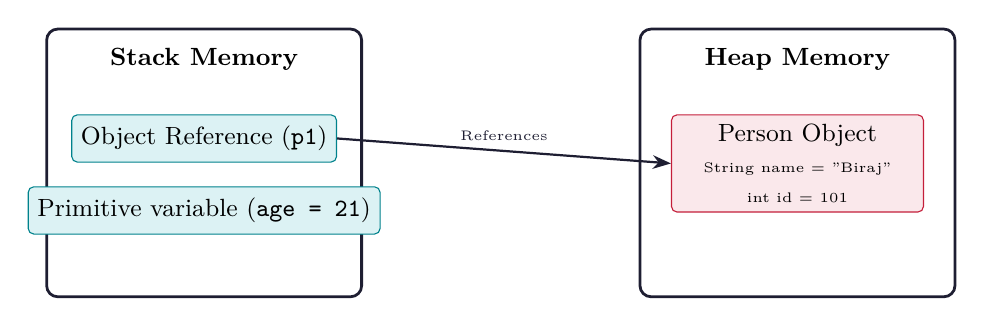
\begin{tikzpicture}[node distance=1.5cm,
  space/.style={rectangle, draw=mydark, line width=1pt, minimum width=4cm, minimum height=3.4cm, rounded corners=4pt},
  element/.style={rectangle, draw=myteal, fill=hdrteal, minimum width=3.2cm, minimum height=0.6cm, font=\small, rounded corners=2pt}]

  % Stack Frame
  \node[space] (stack) {};
  \node[anchor=north, font=\small\bfseries, yshift=-4pt] at (stack.north) {Stack Memory};
  \node[element, below=1.1cm of stack.north] (ref) {Object Reference (\texttt{p1})};
  \node[element, below=0.3cm of ref] (age) {Primitive variable (\texttt{age = 21})};

  % Heap Frame
  \node[space, right=3.5cm of stack] (heap) {};
  \node[anchor=north, font=\small\bfseries, yshift=-4pt] at (heap.north) {Heap Memory};
  \node[rectangle, draw=myred, fill=hdrred, minimum width=3.2cm, minimum height=1.2cm, rounded corners=2pt, below=1.1cm of heap.north, font=\small, align=center] (obj) {Person Object\\{\tiny String name = "Biraj"}\\{\tiny int id = 101}};

  % Connection
  \draw[arrow] (ref.east) -- (obj.west) node[midway, above, font=\tiny] {References};
\end{tikzpicture}
\end{tcolorbox}

\subsection{Control Flow Statements}
Java supports selection (\texttt{if-else}, \texttt{switch}), iteration (\texttt{for}, \texttt{while}, \texttt{do-while}), and jump (\texttt{break}, \texttt{continue}, \texttt{return}) statements:
\begin{itemize}[leftmargin=*, itemsep=3pt]
  \item \textbf{\texttt{break}:} Exits the innermost loop or switch statement immediately.
  \item \textbf{\texttt{continue}:} Skips the current iteration and jumps directly to the next condition evaluation.
  \item \textbf{Labeled Statements:} Loops can be labeled to specify which outer loop a \texttt{break} or \texttt{continue} targets (e.g., \texttt{outerLoop: for(...)}).
\end{itemize}

% ===============================================================================
\section{Class Fundamentals and Variables}
% ===============================================================================

\begin{tcolorbox}[defbox, title={\textbf{Class, Object, and Constructor}}]
\begin{itemize}[leftmargin=*, itemsep=3pt]
  \item \textbf{Class:} A blueprint or template that defines the structure and behaviors (fields and methods) of objects.
  \item \textbf{Object:} A physical instance of a class, holding state values and responding to message calls.
  \item \textbf{Constructor:} A special block of code resembling a method, invoked during object instantiation via the \texttt{new} keyword. It must match the class name exactly and has no return type.
\end{itemize}
\end{tcolorbox}

\subsection{Static vs. Instance Members}
Members marked with the \texttt{static} keyword behave differently from normal instance variables:

\par\noindent
{\renewcommand{\arraystretch}{1.5}%
\begin{tabularx}{\linewidth}{|B{3.2cm}|Y|Y|}
\hline
\textbf{Feature} & \textbf{Static Members} & \textbf{Instance Members} \\
\hline
\textbf{Memory Allocation} & Allocated once in the Metaspace/Method area. & Allocated inside each object on the Heap. \\
\hline
\textbf{Access Syntax} & Accessed via class name (e.g., \texttt{Math.sqrt()}). & Requires an object instance to access. \\
\hline
\textbf{Lifecycle} & Lives from class load to class unload. & Tied to object lifetime; garbage collected. \\
\hline
\textbf{Context} & Cannot reference \texttt{this} or \texttt{super}. & Full access to static and instance members. \\
\hline
\end{tabularx}}

\subsection{Inner Classes}
An inner class is a class declared inside another outer class:
\begin{itemize}[leftmargin=*, itemsep=3pt]
  \item \textbf{Member Inner Class:} Non-static nested class. Holds a reference to the outer class instance and can access all its private members directly.
  \item \textbf{Static Nested Class:} Declared static. Cannot access non-static outer members directly.
  \item \textbf{Anonymous Inner Class:} A class without a name defined inline to implement interfaces or extend abstract classes.
\end{itemize}

\newpage
% ===============================================================================
\begin{center}
  {\large\bfseries\color{myred} Quick Revision --- Module 2}\\[3pt]
  {\small\color{mydark} Introduction to Java Programming \& OOP $|$ OE-EC704A}
\end{center}
\noindent{\color{myred}\rule{\linewidth}{1.2pt}}
\vspace{4pt}

\begin{tcolorbox}[formulabox, title={\textbf{Java Class \& Loop Syntax}}]
{\renewcommand{\arraystretch}{1.3}%
\begin{tabularx}{\linewidth}{l Y}
\textbf{Concept} & \textbf{Syntax and Structural Format} \\
\hline
Class Declaration & \texttt{class Person \{ String name; Person(String n) \{ name = n; \} \}} \\
Main Method Signature & \texttt{public static void main(String[] args) \{ ... \}} \\
Object Instantiation & \texttt{Person p1 = new Person("Biraj");} \\
Static Method Call & \texttt{ClassName.staticMethodName();} \\
\hline
\textbf{Loop Statements} & \textbf{Conditional and Iterative Formats} \\
\hline
\texttt{for} Loop & \texttt{for(initialization; condition; increment/decrement) \{ ... \}} \\
\texttt{while} Loop & \texttt{while(condition) \{ statements; \}} \\
\texttt{do-while} Loop & \texttt{do \{ statements; \} while(condition);} \\
Labeled Break & \texttt{outer: for(...) \{ if(cond) break outer; \}} \\
\end{tabularx}}
\end{tcolorbox}

\begin{tcolorbox}[defbox, title={\textbf{One-Line Definitions}}]
\begin{itemize}[leftmargin=*, itemsep=2pt]
  \item \textbf{JVM (Java Virtual Machine):} An abstract machine that parses and executes compiled Java bytecode.
  \item \textbf{Bytecode:} Standard intermediate instruction format generated by the compiler.
  \item \textbf{JDK:} Comprehensive toolset containing JRE and compiler scripts for developing Java apps.
  \item \textbf{JRE:} Run runtime libraries and JVM package required to execute Java bytecode.
  \item \textbf{Class:} User-defined blueprint declaring structural fields and behavior routines.
  \item \textbf{Object:} An active, stateful runtime instance of a class allocated on the heap.
  \item \textbf{Constructor:} Instantiation routine that initializes object state variables during creation.
  \item \textbf{Garbage Collector:} Automatic JVM system thread that frees heap memory by sweeping unreferenced objects.
\end{itemize}
\tcbset{after={\color{black}}}
\end{tcolorbox}

\begin{tcolorbox}[exambox, title={\textbf{Frequently Asked / Viva Questions}}]
\begin{enumerate}[leftmargin=*, label=\textbf{Q\arabic*.}, itemsep=5pt]
  \item \Q{Why is Java platform-independent but JVM is platform-dependent?}
        Java code compiles to bytecode which runs on any JVM, regardless of the host. However, the JVM must be tailored to the specific OS architecture to translate that bytecode to native machine instructions.
        
  \item \Q{What is the difference between \texttt{path} and \texttt{classpath} variables?}
        \texttt{path} is an OS environment variable locating command-line executables like \texttt{javac} and \texttt{java}. \texttt{classpath} instructs the JVM where to look for compiled user classes and libraries.
        
  \item \Q{Can a class have multiple constructors? If so, how are they distinguished?}
        Yes, this is known as constructor overloading. They are distinguished by their signatures: the number, type, and order of parameters.
        
  \item \Q{What is the default constructor and when is it generated?}
        If no constructor is declared, the compiler automatically generates a no-argument default constructor that initializes fields to default values. If any constructor is declared, this default constructor is not created.
        
  \item \Q{What is the difference between \texttt{break} and \texttt{continue} statements?}
        \texttt{break} exits a loop block immediately, while \texttt{continue} skips only the current iteration and evaluates the loop condition for the next cycle.
        
  \item \Q{What is the purpose of the \texttt{static} keyword in Java?}
        It binds variables or methods to the class itself, rather than to instances. They are loaded once in class metadata space.
        
  \item \Q{Can a static method access non-static instance variables? Why?}
        No. Static methods run without any object instance context, so they do not have access to the \texttt{this} reference necessary to locate instance variables.
        
  \item \Q{What is the difference between pass-by-value and pass-by-reference in Java?}
        Java is strictly pass-by-value. For primitives, a copy of the value is passed. For reference types, a copy of the heap reference address is passed, not the object itself.
        
  \item \Q{What is the purpose of garbage collection in Java?}
        It runs asynchronously to track and reclaim heap memory occupied by objects that have become unreachable from active threads.
        
  \item \Q{Why does Java not support global variables?}
        To prevent global namespace pollution and promote modular encapsulation, Java requires every variable to reside inside a class scope.
\end{enumerate}
\end{tcolorbox}

\begin{tcolorbox}[tikzbox, title={Java Iteration Statement Comparisons}]
\centering
{\renewcommand{\arraystretch}{1.45}%
\begin{tabularx}{\linewidth}{|B{2.8cm}|Y|Y|Y|}
\hline
\textbf{Feature} & \textbf{\texttt{for} Loop} & \textbf{\texttt{while} Loop} & \textbf{\texttt{do-while} Loop} \\
\hline
\textbf{Loop Structure} & Counter-based iteration. & Condition-controlled iteration. & Exit-controlled iteration. \\
\hline
\textbf{Condition Check} & Evaluated at start. & Evaluated at start. & Evaluated at end. \\
\hline
\textbf{Min. Runs} & 0 runs if condition fails. & 0 runs if condition fails. & Guaranteed at least 1 run. \\
\hline
\textbf{Best Use Case} & Iterating when count is known. & Loop until event triggers. & Interactive menus. \\
\hline
\end{tabularx}}
\end{tcolorbox}

\end{document}
